Our solution have three machine learning (ML) component, Speech to Text, Chatbot, and Text to Speech.
Representing sounds or human voice in digital media involves converting them into analog signals.
The main challenge lies in converting these analog signals into text format, which enables machines to process and work with the data effectively and the Speech to Text solves this problem \cite{speech-recog-bengali}.
A Chatbot is a computer program or an artificial intelligence which conducts a conversation via auditory or textual methods \cite{chatbot}.
Text-to-Speech (TTS) is a technology that converts written text into spoken words \cite{text-to-speech}.

Figure \ref{fig:methodology} shows a user provide a voice input, then our system process the voice data and provide that data into Speech to Text.
Speech to Text returns text data for the voice data, this data is the input of the chatbot, chatbot takes the decision, like what to do, what to reply, or what to ask, these kind of questions.
If the response is to take an action based on the output of the chatbot, then it takes the action, like call someone, interaction with IoT devices etc.
Also, provide the voice feedback to the user using Text to Speech.
There are a plenty of solutions for other top languages, but we have developed for Bengali language.

\begin{figure}
    \centering
    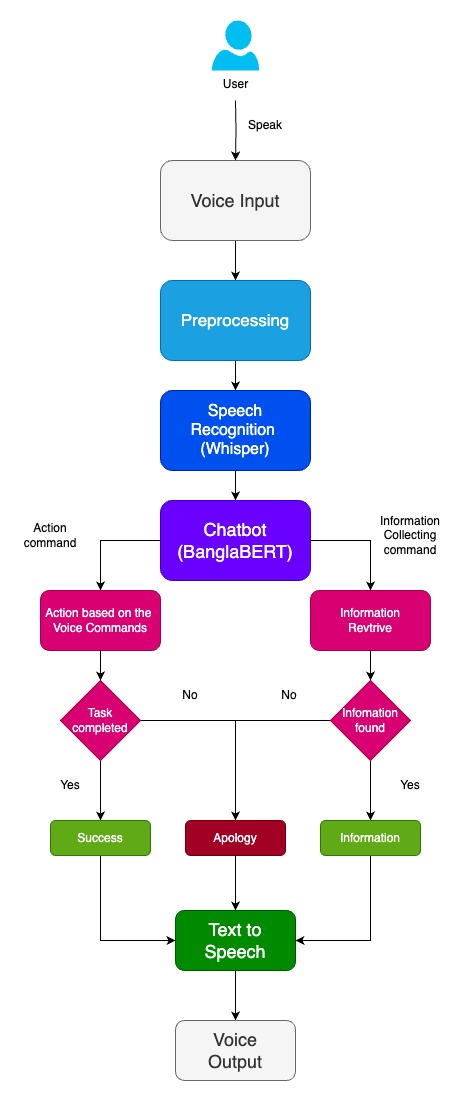
\includegraphics[width=0.4\textwidth]{Methodology-diagram}
    \caption{System Architecture of the proposed solution}\label{fig:methodology}
\end{figure}

Our deployment environment (Figure \ref{fig:deployment}) is in the cloud, using API access a mobile/computer app can interact with the system.
A basic model will be downloaded into the local device as well to make the communication with reduced latency.
When a user provide some basic voice command the local model will be sufficient to reply or interact with that.
But when a complex or unknown reply is required then it will communicate with the cloud version of the model.
The models are self improvable, for example it will learn to understand a specific user in a better way by user's feedback and Reinforcement Learning (RL).
Also, the local model is trained with the most commonly used commands, so that it can respond quickly for the most common words for a specific user.

\begin{figure}
    \centering
    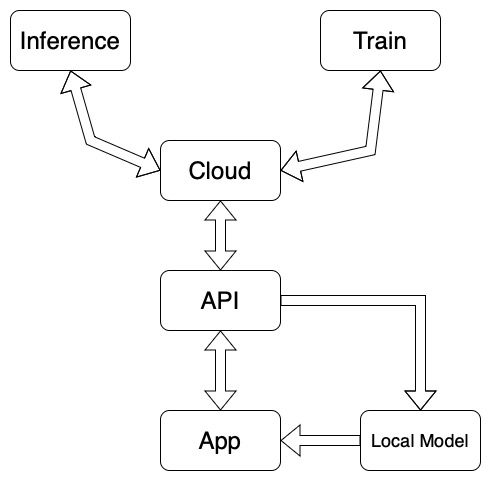
\includegraphics[width=0.4\textwidth]{Deployment}
    \caption{Deployment architecture of the system}\label{fig:deployment}
\end{figure}
